% The entire content of this work (including the source code
% for TeX files and the generated PDF documents) by 
% Hongxiang Chen (nicknamed we.taper, or just Taper) is
% licensed under a 
% Creative Commons Attribution-NonCommercial-ShareAlike 4.0 
% International License (Link to the complete license text:
% http://creativecommons.org/licenses/by-nc-sa/4.0/).
\documentclass{book}

\usepackage{float}  % For H in figures
\usepackage{amsmath, amssymb} % For math
\usepackage{mathtools} % dcases*, see https://en.wikibooks.org/wiki/LaTeX/Advanced_Mathematics#The_cases_environment
\numberwithin{equation}{subsection} % have the enumeration go to the subsection level.
% See:https://en.wikibooks.org/wiki/LaTeX/Advanced_Mathematics
\usepackage{graphicx}   % need for figures
\usepackage{cite} % For bibligraphy
\usepackage{fancyref} % For lazy reference \fref
\usepackage[unicode]{hyperref} % For hyperlink everything.
\usepackage{CJKutf8} % For Chinese characters
%\usepackage{ dsfont } % For double struck fonts
\usepackage{braket} 
\usepackage[T1]{fontenc}
\usepackage{listings}

\usepackage{amsthm}
\newtheorem{defi}{Definition}[section]
\newtheorem{thm}{Theorem}[section]
\newtheorem{lemma}{Lemma}[section]
\newtheorem{remark}{Remark}[section]
\newtheorem{prop}{Proposition}[section]
\newtheorem{coro}{Corollary}[section]
\theoremstyle{definition}
\newtheorem{ex}{Example}[section]

\usepackage{tensor}  % For tensor indices
\usepackage[all]{xy} % For drawing category diagrams
\usepackage{mathrsfs}

\title{Notes of Quantum Field Theory in a Nutshell}
\date{\today}
\author{we.taper}
\begin{document}
	\maketitle
	\tableofcontents

\chapter{Part I: Motivation and Foundations}
\label{sec:QFT_in_a_Nutshell.Part_I}
\section{I.2 Path Integral Formulation of Quantum Physics}
\label{sec:QFT_in_a_Nutshell_Part_I.2}
Here the path integral formulation of quantum mechanics is introduced.
The intuition comes from a limiting case of the traditional double 
slit electron interference experiment. (\textbf{pp.7 to 10}) Then 
it calculates the transition probability $\braket{q_F|e^{-iHT}|q_I}$
by divide it into a infinite of steps:
\begin{align}
    \braket{q_F|e^{-iHT}|q_I} = \lim_{N\to \infty}
    \braket{q_F|e^{iH\delta t}e^{iH\delta t}\cdots e^{iH\delta t}|q_I}
    (\text{with }N\delta t = T)
\end{align}

For illustration, it calculates this value when 
$H=\frac{\hat{p}^2}{2m}$. The result is that:
\begin{align*}
    \braket{q_F|e^{-iHT}|q_I} = \int Dq(t) 
        e^{i\int_0^T dt \frac{1}{2}m \dot{q}^2 }
\end{align*}

where:
\begin{align}
    \int Dq(t) \equiv \lim_{N\to \infty} 
    \left( \frac{-im}{2\pi \delta t}\right)^{N/2}
    \left( \prod_{k=1}^{N-1} \int dq_k \right)
\end{align}
It notes that when $H=\hat{p}^2/2m + V(\hat{q})$, the final result
would have been:
\begin{align}
    \label{eq:QFT_in_a_Nutshell_Part_I.2.TransProbability}
    \braket{q_F|e^{-iHT}|q_I} &= \int Dq(t) 
        e^{i\int_0^T dt \frac{1}{2}m \dot{q}^2 - V(q)}
        \nonumber \\
        &=\int Dq(t) e^{i \int_0^T dt L(\dot{q}, q)}
\end{align}
where $L$ is the Lagrangian of the system.

Often, the value we need to calculate is $\braket{F|e^{-iHT}|I}$.
Using $\int \ket{q}\bra{q} dq=1$, we have:
\begin{align}
    \braket{F|e^{-iHT}|I} = \int dq_F \int dq_I
        \braket{F|q_F} \braket{q_F|e^{-iHT}|q_I}\braket{q_I|I}
\end{align}

The value \(\braket{0|e^{-iHT}|0}\) is denoted $Z$. This part
mentions that one often effect a change of coordinate
$t \to -it$, called \textit{Wick rotation}, to obtain:
\begin{align}
    Z = \int Dq(t) e^{-\int_0^T dt H(\dot{q},q)}
\end{align}
where $H$ is the Hamiltonian of the system.
The mathematical rigorous aspect is often ignored.

It also discuss how this formulation could explain the classical
limit of quantum mechanics, i.e. classical mechanics, in a
very direct manner. This is related to the saddle point
approximation to the integral 
\ref{eq:QFT_in_a_Nutshell_Part_I.2.TransProbability}.

\textbf{Unclear point}
Why is $\int dq \ket{q}\bra{q} = 1$ while $\int \frac{p}{2\pi}
\ket{p}\bra{p} = 1$. What does it mean by saying
"to see that the normalization is correct" (pp. 10 and 11).
Why is effecting the Wick rotation is "somewhat rigorous"?

\textbf{Corresponding pages in draft} pp. 1 to 3.

    \subsection{Appendix 1 - Dirac Delta function and
        \texorpdfstring{$\varepsilon$}{} as infinitesimal
        small value}

    Here the Dirac Delta function is defined as the limit of another
    function $d_K(x)$. Since:
    \begin{align}
        d_K(x) \equiv \int_{-K/2}^{K/2} \frac{dk}{2\pi} e^{ikx} = 
            \frac{1}{\pi x}\sin\frac{Kx}{2}\\
        \int_{-\infty}^{\infty} dx\text{ } d_K(x) = 1
    \end{align}
    Hence we de fine $\delta(x) = \lim_{K\to \infty}d_K(x)$.
    Other important formula include:
    \begin{align}
        \delta(x) = \int_{-\infty}^{\infty} \frac{dk}{2\pi}e^{ikx} \\
        \frac{1}{x+i\varepsilon} = \mathcal{P}\frac{1}{x}-i\pi \delta(x)\\
        \delta(x) = \frac{1}{\pi}\frac{\varepsilon}{x^2+\varepsilon^2}
    \end{align}
    Here $\varepsilon$ is a infinitesimal value. $\mathcal{P}$ denotes the
    principal value integral, defined by:
    \begin{align}
        \int dx \mathcal{P}\frac{1}{x}f(x) = \lim_{\varepsilon\to 0}
            \int dx \frac{x}{x^2+\varepsilon^2}f(x)
    \end{align}
    \subsection{Appendix 2 - Wick theorem in Gaussian 
    Integral}

    This part introduces some very important formulae, listed 
    below:

    (It is very important that $A$ is a real symmetric matrix.)
    
    \begin{align}
        &\int_{-\infty}^{+\infty} \int_{-\infty}^{+\infty} \cdots
        \int_{-\infty}^{+\infty} dx_1 dx_2 \cdots dx_N
            e^{-\frac{1}{2} x^T A x + J^T x} =
            \left( \frac{(2\pi)^N}{\text{det}A} \right)^{\frac{1}{2}}
            e^{\frac{1}{2}J^T A^{-1}J}
   		\label{eq:QFT_in_a_Nutshell_Part_I.2.appdx1.1}
		\\
        &\int_{-\infty}^{+\infty} dx
        e^{-\frac{1}{2}ax^2+Jx} =
        \left(\frac{2\pi}{a}\right)^{\frac{1}{2}}
        e^{\frac{J^2}{2a}} 
        \\
        &\braket{x_i x_j \cdots x_k x_l}
        \equiv
            \frac{
                \int_{-\infty}^{+\infty}\int_{-\infty}^{+\infty}\cdots
                \int_{-\infty}^{+\infty} dx_1 dx_2\cdots dx_N
                e^{-\frac{1}{2}x^T Ax} x_i x_j \cdots x_k x_l}
                {
                \int_{-\infty}^{+\infty}\int_{-\infty}^{+\infty}\cdots
                \int_{-\infty}^{+\infty} dx_1 dx_2\cdots dx_N
                e^{-\frac{1}{2}x^T Ax} }
            \nonumber \\
        &= \sum_{\text{Wick}} 
            (A^{-1})_{ab}\cdots(A^{-1})_{cd}
    \end{align}
    For example:
    \begin{align*}
        &\braket{x^{2n}} \equiv 
            \frac{\int_{-\infty}^{+\infty}dx
            e^{-\frac{1}{2}ax^2} x^{2n}}
            {\int_{-\infty}^{\infty} dx e^{-\frac{1}{2}ax^2}
            }
        = \frac{1}{a^n}(2n-1)!! \\
        &\braket{x_ix_jx_kx_l} = 
        (A^{-1})_{ij}(A^{-1})_{kl}+(A^{-1})_{ik}(A^{-1})_{jl}
        +(A^{-1})_{il}(A^{-1})_{jk}
    \end{align*}
    \textbf{Corresponding pages in draft} pp. 4 to 6.
    
\section{I.3 From Mattress to Field}
\label{sec:QFT_in_a_Nutshell_Part_I.3}
\paragraph{Note} After reading this section and several comments online,
I realize that this book put more emphasize on physical
intuition than on mathematical rigor. To illustrate this point, I
quote a sentence from A. Zee's homepage at UCSB, which comes from
a review of this book (QFT in a Nutshell):

\begin{quote}
    "It is often deeper to know why something is true rather than to have a proof that it is true."
\end{quote}

By above reason, I gave up tracking the calculations done in this
book.

\paragraph{Mattress in continuum limit} It start with taking the
limit of lattice spacing $l\to 0$, aiming to write down the field
equation from the mattress perspective. The process is transparant
and neatly summarized in the "promotion table" on page 19:

\begin{center}
\begin{tabular}{| c | c |}
    \hline
    function  & $q\to \phi$  \\
    \hline
    atom position  & \(a\to x\)  \\
    \hline
    dynamic function  & \(q_a(t) \to \phi(t,\mathbf{x})=\phi(x)\)  \\
    \hline
    summation  & \(\sum_a \to \int d^D x\)  \\
    \hline
\end{tabular}
\end{center}

In detail, $\sum_a \frac{1}{2} m_a\dot{q}_a^2$ becomes 
$\int d^2x \frac{1}{2} \sigma (\partial \phi/\partial t)^2$.,
$\sum_{ab} k_{ab} \frac{1}{2} (q_a-q_b)^2$ becomes
$\int d^2x \rho( \frac{\partial^2 \phi}{\partial x^2}
    + \frac{\partial^2 \phi}{\partial y^2})$, and

\begin{align}
    S(q) &\to S(\phi) \equiv \int_0^T dt \int d^2x \mathcal{L}(\phi)
    \nonumber \\
    &= \int_0^T dt \int d^2x \frac{1}{2}
    \left\lbrace \sigma ( \frac{\partial \phi}{\partial t})^2
    -\rho \left[ ( \frac{\partial \phi}{\partial x})^2 +
        \frac{\partial \phi}{\partial x})^2 \right]
    -\tau\phi^2 -\xi\phi^4 +\cdots \right\rbrace
\end{align}

% TODO why not odd terms
Then he notes about the Landau-Ginzburg view:

\begin{quote}
    we start with the desired symmetry, say Lorentz invariance if we
    want to do particle physics, decide on the fields we want by 
    specifying how they transform
    under the symmetry (in this case we decided on a scalar field 
    $\phi$), and then write down
    the action involving no more than two time derivatives 
    (because we don’t know how to
    quantize actions with more than two time derivatives)
\end{quote}

Also it is customary to write $d = D + 1$ and speak of a 
$(D + 1)$-dimensional spacetime. When $D=0$, quantum
field theory reduces to normal quantum mechanics,
which deal with only a point (in the mattress
sense, we have only one particle).

Then he also notes that the Lagrangian can only have the form
$\mathcal{L}=\frac{1}{2}(\partial\phi)^2-V(\phi)$.\footnote{
    in a footnote, he also mentions a possible additional
    term $U(\phi)(\partial \phi)^2$. It is related to a
    particle whose mass depends on position. This will be
considered later}.

The classical limit of this formulation can be obtained by
method similar to previous section. A saddle point approximation
to the integral:
\begin{align}
    Z = \int D\phi e^{i/\hbar \int d^4x \mathcal{L}(phi)}
\end{align}
will find the classical field equation:
\begin{align}
    \label{eq:QFT_in_a_Nutshell_Part_I.3.classicalFieldEq}
    \partial_\mu \frac{\delta \mathcal{L}}{\delta(\partial_\mu\phi)}
    -\frac{\delta\mathcal{L}}{\delta\phi} =0
\end{align}

\textbf{Corresponding pages in draft} pp. 7 to 8.

\paragraph{Vacuum and Response}

It is said that the vacuum in quantum field theory is a
stormy sea of quantum fluctuations.

Then, it discuss a process, very similar to the idea in linear
response theory in condensed matter physics. The idea is to
set up a source and a sink in which particles are created and
annihilated. It correspondes to adding a term $sum_a J_a(t)q_a$ to
the potential, or in the continuum limit, a term $\int d^DxJ(x)\phi(x)$.

\paragraph{Free field theory}

Here he centers at the the Lagrangian
\begin{align}
    \mathcal{L}(\phi)=\frac{1}{2}\left( (\partial\phi)^2-m^2\phi^2\right)
\end{align}
The corresponding theory is called the \textbf{free} or 
\textbf{Guassian theory}. Using 
% TODO why is it called free
\ref{eq:QFT_in_a_Nutshell_Part_I.3.classicalFieldEq}, one can easily
obtain the Klein-Gorden equation:
\begin{align}
    (\partial^2+m^2)\phi=0
\end{align}
The plain wave solution is of the form:
\begin{align}
    \omega^2=\vec{k}^2+m^2
\end{align}
He notes that by transfer back to the SI unit, one will
recognize above equations the same as the $E=mc^2$ identity.

Next, we evaluate the disturbed case of free field theory:
\begin{align}
    Z = \int D\phi e^{i\int d^4x \left( \frac{1}{2} 
        [(\partial\phi)^2-m^2\phi^2]+J\phi \right)
        }
\end{align}
The integration is rather lengthy. It involves a trick called
"to imagine discretizing spacetime". In my opinion, such a trick
is to the best, a fancy intuition. There maybe mathematical proof,
but is neglected by the author. However, the result is surprisingly
rich in intuition and analogy. It start with the discretized
analogy with \eqref{eq:QFT_in_a_Nutshell_Part_I.2.appdx1.1}. One
is gradually lead to believe that the result of:
\begin{align}
    Z = \int D\phi e^{ i\int d^4x 
        \left(-\frac{1}{2}(\partial^2+m^2)\phi+J\phi \right)}
\end{align}
is:
\begin{align}
    \label{eq:QFT_in_a_Nutshell_Part_I.3.3}
    Z(J) = \mathcal{C}e^{-(i/2) \int\int d^4xd^4y J(x)D(x-y)J(y)}
\end{align}
where $\mathcal{C}$ is just some factor which will proven to be
unimportant. $D(x-y)$ is the solution of:
\begin{align}
    \label{eq:QFT_in_a_Nutshell_Part_I.3.2}
    -(\partial^2+m^2)D(x-y)=\delta^{(4)}(x-y)
\end{align}

The following is devoted to the function $D(x)$.

One checks by direct substitution that:
\begin{align}
    D(x-y) = \int \frac{d^4k}{(2\pi)^4} 
        \frac{e^{ik(x-y)}}{k^2-m^2+i\varepsilon}
\end{align}
is the solution to \ref{eq:QFT_in_a_Nutshell_Part_I.3.2}.

We also denote the exponent in \ref{eq:QFT_in_a_Nutshell_Part_I.3.3}
as $W(J)$. So:
\begin{align}
    \label{eq:}
    W(J) = -\frac{1}{2} \int\int d^4x d^4y J(x)D(x-y)J(y) \\
    Z= \mathcal{C}e^{iW(J)}
\end{align}

\paragraph{Free propagator}

The function $D(x)$ is also called a propagator. It "plays an 
essential role in quantum field theory. As the inverse of a
differential operator it is clearly closely related to the Green’s
function you encountered in a course on electromagnetism".

Then the author tries to explain how to evaluate $D(x)$, which
I fail to reproduce. The final result is equation (23) on page 
24:
\begin{align}
    D(x)= -i\int \frac{d^3k}{(2\pi)^3 2\omega_k}
    \left( e^{-i(w_k t-\vec{k}\cdot\vec{x})} \theta(x^0)
        + e^{i(w_k t-\vec{k}\cdot\vec{x})} \theta(-x^0)
    \right)
\end{align}

He notes that
\begin{quote}
    Physically, $D(x)$ describes the amplitude for a disturbance 
    in the field to propagate from the origin to $x$. 
\end{quote}
In different region of spacetime, the value of $D(x)$ varies greatly.
When $x$ is in timelink region, $D(x)$ is the superposition of
plane waves, while the phase is opposite between $x^0=t<0$ and
$x^0=t>0$. When $x$ is in the spacelike region, the $D(x)$ exhibits
a strange behavior that the particle can leak outside lightcone,
over a distance of order $m^{-1}$. This is consistent with the
Heisenberg's uncertainty principle.

\textbf{Corresponding pages in draft} pp. 9 to 11.

\textbf{Unclear points}: I cannot follow all the calculation for 
$D(x)$, because my result is different from the book's. Also, the
physics picture about $D(x)$ on page 24, is badly reasoned. The
argument is tenuous, in my opinion.

\section{I.4 From Field to Particle to Force}
\label{sec:I.4 From Field to Particle to Force}

\textbf{Note}: discussion in this section is based on the \textit{free
field theory}.

\paragraph{From field to particle}

With the Fourier transformation, several physical properties
could be extrated from $W(J)$. The Fourier transformed $W(J)$ is:
\begin{align}
    W(J) = -\frac{1}{2}\int \frac{d^4}{(2\pi)^4}J(k)^*
        \frac{1}{k^2-m^2+i\epsilon}J(k)
\end{align}
If separating $J$ into $J(x)=J_1(x)+J_2(x)$, then naturally, the
Fourier transformed calculation will include terms of the form:
$J^*_1J_1,J^*_1J_2,J^*_2J_1,J^*_2J_2$. We see that the denominator
in $W(J)$ contains $k^2-m^2$. Somehow the author wants to argue that
the term $J^*_2J_1$ describes the influence of a particle of mass $m$
propagating from the source $1$ to the sink $2$. But his language is loose.

This part also introduces the jargon \textit{on mass shell} and the
language of "virtual particles" moving in $k$-space.

\paragraph{From particle to force}
With two delta source $J_a(x)=\delta^(3)(\vec{x}-\vec{x}_a)$, one can
describe two massive lumps setting on $\vec{x}_1$ and $\vec{x}_2$ and
not moving at all. These two lumps, coupled with the free field $\phi$,
will attract each other. To show the attraction, the author calculates
explicitly the $W(J)$, and identifies $iW(J) \equiv -iET$ (the
identification is substantiate by $e^{-iET} = Z = e^{iW(J)}$).
Finally, it shows:
\begin{align}
    E= -\frac{1}{4\pi r}e^{-mr}
\end{align}
This is actually the Yukawa model for the attraction between nucleons
in the atomic nucleus. A plot is in due:
\begin{figure}[H]
    \centering
    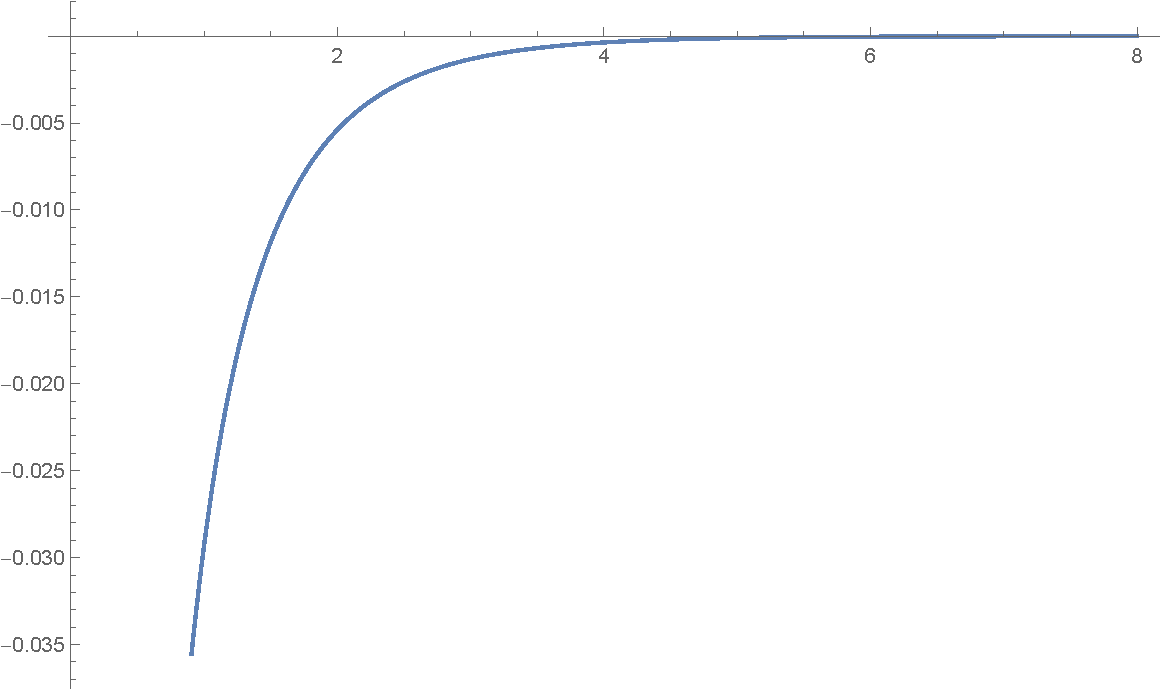
\includegraphics[width=0.8\linewidth]{pics/Yukawa-potential.pdf}
    \caption{Plot of Yukawa potential $-\frac{e^{-r}}{4 \pi  r}$}
\end{figure}

It shows us several information:
\begin{itemize}
    \item In the long distance, the potential drops off over the
        distance scale of $1/m$.
    \item In the short range, the force is $1/r^2$.
    \item The energy gets smaller when the two sources come closer.
        It tends to $-\infty$ as $r\to 0$.
\end{itemize}

\paragraph{Origin of force}
% TODO stops here.
\chapter{Bibliography}
\begin{thebibliography}{1}
	\bibitem{zee} A. Zee. Quantum Field Theory in a Nutshell
		2ed. PUP.
\end{thebibliography}
\chapter{License}
The entire content of this work (including the source code
for TeX files and the generated PDF documents) by 
Hongxiang Chen (nicknamed we.taper, or just Taper) is
licensed under a 
\href{http://creativecommons.org/licenses/by-nc-sa/4.0/}{Creative 
	Commons Attribution-NonCommercial-ShareAlike 4.0 International 
	License}. Permissions beyond the scope of this 
license may be available at \url{mailto:we.taper[at]gmail[dot]com}.


\end{document}
